\documentclass{scrartcl}
\usepackage{pgfplots}
\usepackage{graphicx}
\usepackage{pgfplotstable}
\usepackage{csvsimple}
\usepackage[left=1cm, right=1cm, top=1cm, bottom=3cm]{geometry}

\usepackage{titlesec}
\usepackage{xcolor}
\usepackage{background}
\backgroundsetup{
scale=1,
angle=90,
opacity=0,
contents={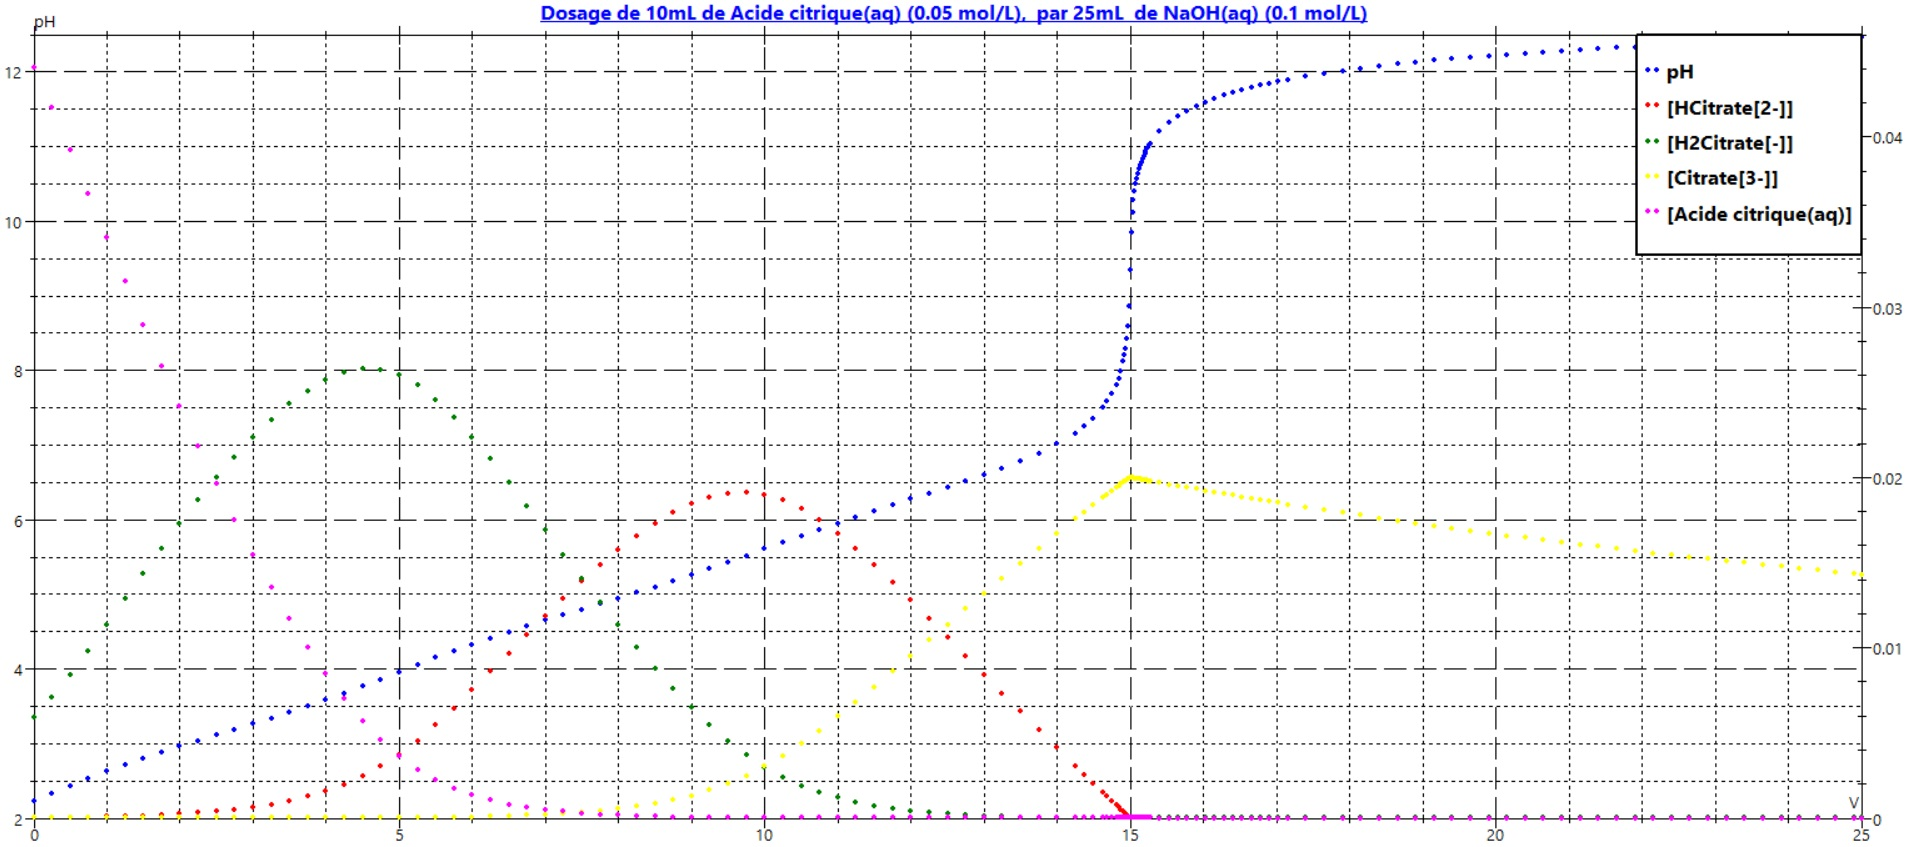
\includegraphics[width=\paperwidth,height=\paperheight,keepaspectratio]{polyacide.jpg}}
}
\titlelabel{\thetitle\quad}
\setlength{\parindent}{0pt}

\newcommand\courbe[1]{

\begin{tabular}{@{}cc@{}}
			
				\begin{tabular}{l|c}%
					\bfseries v (en mL) & \bfseries pH
					\csvreader[head to column names]{data/courbe#1.csv}{}
					{\\\hline\x & \y}
				\end{tabular}
				
				\begin{tabular}{l|c}%
					\bfseries v (en mL) & \bfseries $\mathbf{\frac{\partial pH}{\partial v}}$
					\csvreader[head to column names]{data/courbeDerivative#1.csv}{}
					{\\\hline\x & \y}
				\end{tabular}

				\pgfplotstableread[col sep = comma]{data/courbe#1.csv}\ph
				\pgfplotstableread[col sep = comma]{data/courbeDerivative#1.csv}\dph

				\begin{tikzpicture}
					\begin{axis}[
						xlabel=$v$ (en mL),
						ylabel=$\textcolor{red}{pH}$]
						\addplot[color = red, mark = x] table {\ph};
					\end{axis}
					\pgfplotsset{every axis y label/.append style={rotate=0,yshift=-9.5cm}}
					\begin{axis}[axis y line*=right, hide x axis, ylabel=$\textcolor{blue}{\frac{\partial pH}{\partial v}}$]
						\addplot[color = blue, mark = x] table {\dph};
					\end{axis}
				\end{tikzpicture}
				
		\end{tabular}\\
		
}

\begin{document}

	\title{\vspace{-2cm}Compte-rendu de travaux pratiques de chimie}
	\subtitle{Dosages acido-basique de polyacides}
	\author{Benjamin Loison (MPSI 1)}
	\date{}
	\maketitle

  %\setcounter{section}{2}
	%\section{Utilisation du pH-mètre}
	
		
	\setcounter{section}{3}
	\section{Tracé de courbes de dosages acido-basiques}
	
		\subsection{Dosage d'une solution d'acide phosphorique par la soude}
			
				\courbe{1}
			
				On a les trois pKa suivants:\\
				pKa($H_3PO_4/H_2PO_4^-$) = 2.2\\
				pKa($H_2PO_4^-/HPO_4^{2-}$) = 7.2\\
				pKa($HPO_4^2-/PO_4^{3-}$) = 12.3.\\
				
				En travaillant avec la dérivée instantanée des ordonnées de la courbe ci-dessus, on remarque deux sauts de pH:\\
				- de 3.39 à 5.16 entre 4.5 mL et 5 mL.\\
				- de 8.43 à 10.24 entre 10 et 10.5 mL.\\
				
				On note $c$ la concentration de l'acide et $c_1$ celle de la soude.
				A la première équivalence, on a alors: $cv = c_1v_{eq}$, donc $c = \frac{c_1v_{eq}}{v} = \frac{0.1 * 4.75}{10} = 0.0475$ mol/L.\\
				A la seconde équivalence, on a alors: $c = \frac{0.1 * 10.25}{2 * 10} \approx 0.05125$ mol/L.\\
				La verrerie nous indique, une incertitude sur chaque mesure de volume d'environ 0.04 mL.\\
				On calcule ensuite $\Delta c = c\sqrt{\left(\frac{\Delta c_1}{c_1}\right)^2 + \left(\frac{\Delta v_{eq}}{v_{eq}}\right)^2 + \left(\frac{\Delta v}{v}\right)^2} = 3 * 10^{-3}$ mol/L\\
				De même pour le second, on obtient: $\Delta c = 1.3 * 10^{-3}$ mol/L.\\\\
				
				A la première demi-équivalence, le pH vaut environ 2.6, ce qui est légèrement supérieur au $pK_1$ selon la première courbe et le second vaut approximativement 7.05. Les écarts relatifs associés sont alors: $\frac{|2.2 - 2.6|}{2.2} \approx$ 0.18 et $\frac{7.2 - 7.05}{7.2} \approx$ 0.02.\\\\
				
				Les deux équations de titrage sont:\\
				
				$H_3PO_4 + HO^- \rightleftharpoons H_2PO4^- + H_2O$\\
				$H_2PO_4^- + HO^- \rightleftharpoons HPO4^- + H_2O$\\
				Et on a respectivement:\\
				$pK_1 = 2.2$\\
				$pK_2 = 7.2$\\
				
				On a donc le rapport $\frac{K_1}{K_2} = 10^{7.2 - 2.2} = 10^5$, avec cette valeur élevée, on peut alors assimiler les titrages à des titrages successifs.
						
		\subsection{Dosage d'une solution d'acide citrique par la soude}
			
			\courbe{2}
			
			On a les 4 pKa suivants:\\
			$pKa(H_4Cit/H_3Cit^-) = 3.1$\\
			$pKa(H_3Cit^-/H_2Cit^{2-}) = 4.7$\\
			$pKa(H_2Cit^{-2}/HCit^{3-}) = 6.4$\\
			$pKa(HCit^{3-}/Cit^{4-}) = 16$\\
			La forme basique $Cit^{4-}$ ne peut pas exister dans l'eau pure, elle est immédiatement dissociée. On ne peut donc pas montrer les 3 sauts de pH dans l'eau pure.\\\\
			
			On remarque avec la dérivée instantanée du pH en fonction du volume versée, deux sauts de pH:\\
			- de 6.73 à 7.63 entre 14.5 mL et 15 mL.\\
			- de 7.63 à 10.41 entre 15 mL et 15.5 mL.\\
			
			Le premier saut est associé aux deux premières acidités, dont les pKa sont trop proches pour que les titrages soient considérés comme successifs.\\
			Le second saut montre clairement la troisième acidité de pKa 6.4. Le pH a dû monter très vite dans la zone de virage de la phénolphtaline après le passage de la troisième acidité, cela explique pourquoi on observe un changement de couleur de la solution avec un ajout de seulement 0.5 mL de soude.
			\newpage
			\underline{Aperçu du dosage sur Dozzaqueux:}
			\backgroundsetup{
scale=1.25,
angle=90,
opacity=1,
contents={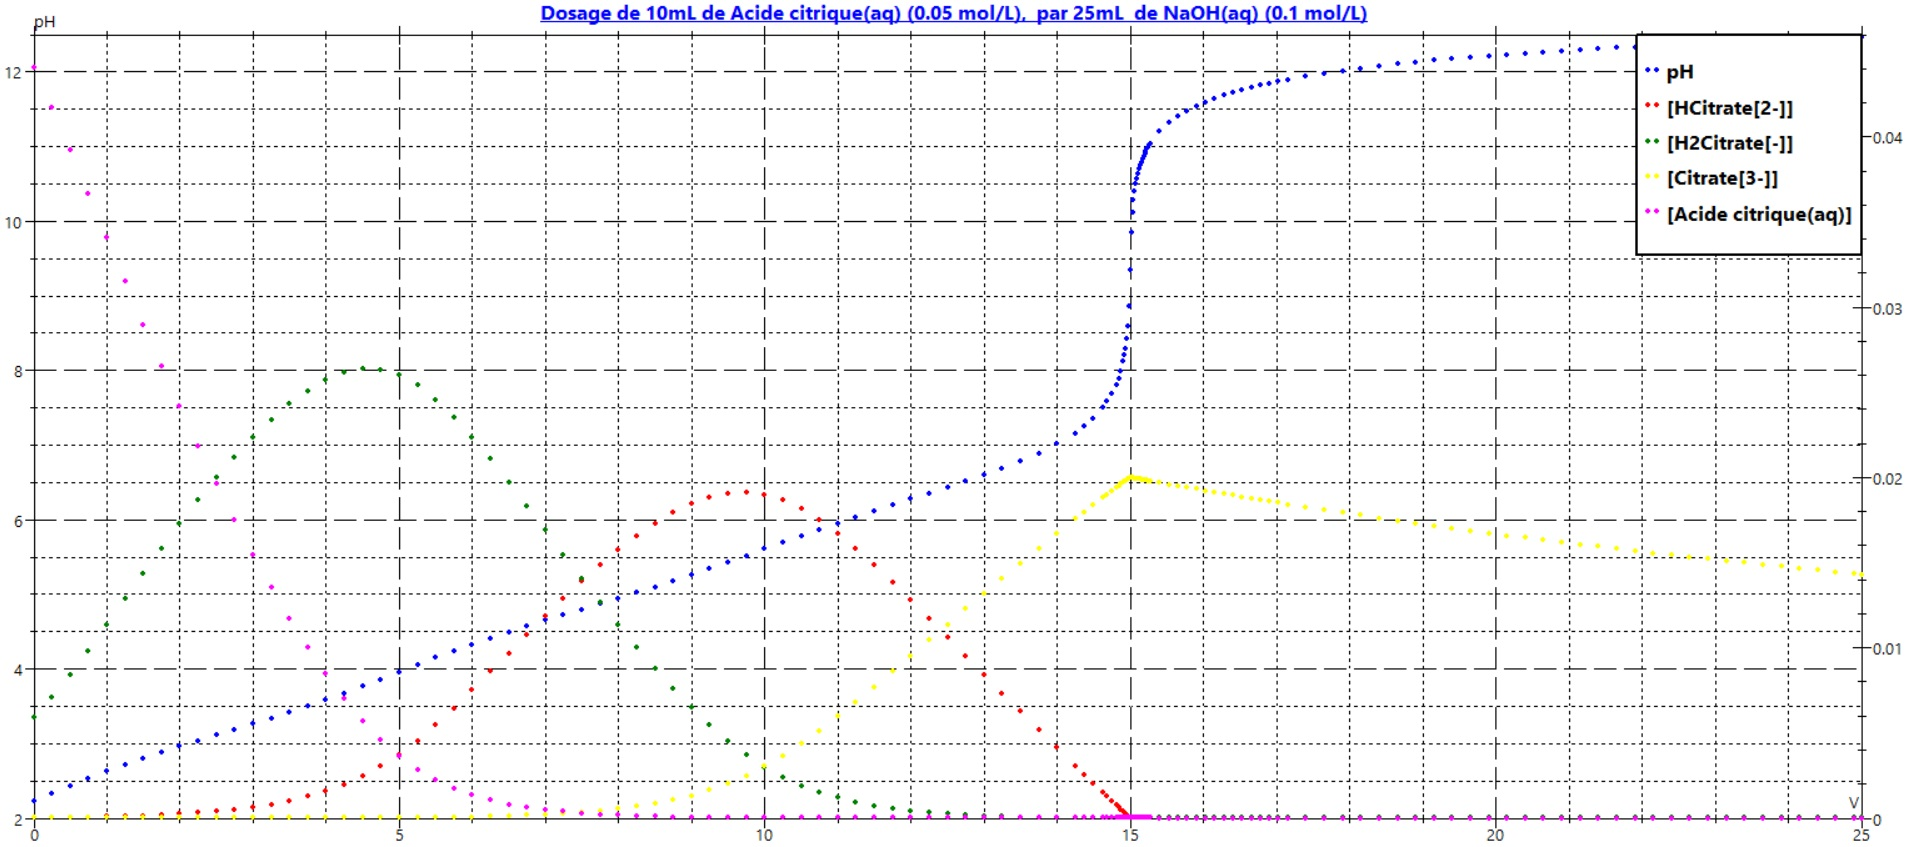
\includegraphics[width=\paperwidth,height=\paperheight,keepaspectratio]{polyacide.jpg}}
}
			
		%\subsection{Utilisation d'un logiciel de simulation}	
			
			% courbe dozaqueux
			
\end{document}